\chapter{Introduction}

With the threat of anthropogenic climate change and the looming end to fossil
fuel supplies, human civilization must reduce carbon emissions \cite{Hansen2013}
and transition to a fully sustainable energy portfolio. Towards this end,
natural fluid flows such as wind and water in river and tidal flows---a.k.a.
marine hydrokinetic (MHK) energy---can contribute. It is estimated that there is
still \todo[inline]{Find how much untapped wind energy there is} W of wind power
left untapped globally, while there is approximately 50 GW of technically
available MHK power in the US \cite{Haas2011, Jacobson2012, Haas2013}. For
reference, the US used about 450 GW of electricity on average in XXXX
\todo[inline]{Get citation for US energy use and add a year.}.

A turbine is the most common machine for extracting energy from these flows,
converting the energy to shaft work by the fluid applying torque on the rotor.
Wind turbine designs have matured a lot over the past couple decades, to the
point where they are not changing much conceptually, though they are pushing
forward by increasing size. MHK turbine designs on the other hand are quite
immature despite taking heavy influence from wind technology.

Turbine rotor concepts can essentially be divided into two classes---axial-flow
and cross-flow---describing the relative orientation of the axis to the nominal
flow direction. The ubiquitous horizontal-axis wind turbine (HAWT) is an example
of an axial-flow turbine (AFT), while the egg-beater shaped Darrieus
vertical-axis wind turbine (VAWT), patented in 1931 \cite{Darrieus1931}, is an
example of a cross-flow turbine (CFT). Note that a cross-flow turbine can accept
flow from any direction perpendicular to its rotation, meaning the axis can be
horizontal, vertical, or anything in between.

The most well-know CFT, the Darrieus vertical-axis wind turbine, examples of
which are shown in Figure~\ref{fig:Darrieus}, was developed thoroughly in the
late 1970s through the early 1990s by groups including Sandia National
Laboratories (SNL) in the US and the National Research Council (NRC) in Canada
\cite{Para2002}. Sandia's efforts culminated in their 34 m Test Bed, shown in
Figure~\ref{fig:Sandia-34m}. The lessons and knowledge gained from this research
turbine were used to create a ``point design'' for commercialization
\cite{Sutherland2012}. Turbine developer FloWind used the point design and
technical guidance from SNL to develop three-bladed composite rotors for their
fleet of VAWTs, shown in Figure~\ref{fig:FloWind}, resulting in moderate
commercial success. The highest power output of any VAWT---in the 1--3 MW
range---was achieved by the Canadian Lavalin Eole 64 m Research Turbine,
constructed in 1986 \cite{Para2002}, and shown in Figure~\ref{fig:Eole}.

\begin{figure}
    \centering

    \begin{subfigure}[b]{0.58\textwidth}
        \centering
        
        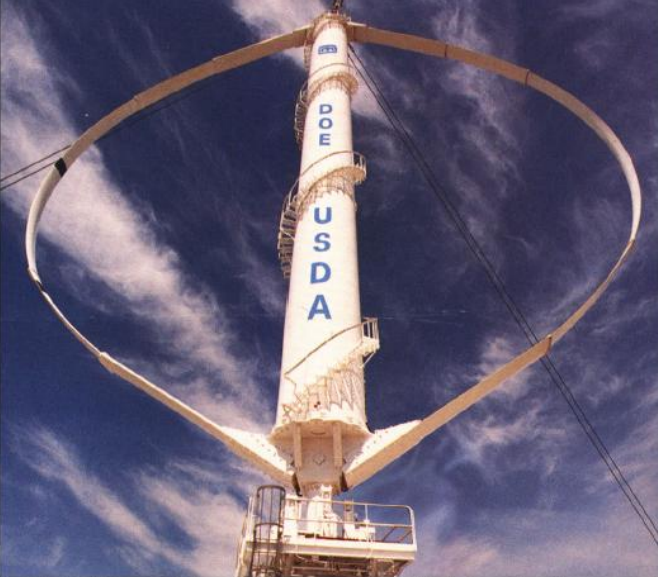
\includegraphics[width=\textwidth]{Murray2011-34m}
        
        \caption{Sandia 34 m Test Bed, from \cite{Murray2011}.}
        
        \label{fig:Sandia-34m}
    \end{subfigure}
    \hfill
    \begin{subfigure}[b]{0.365\textwidth}
        \centering
        
        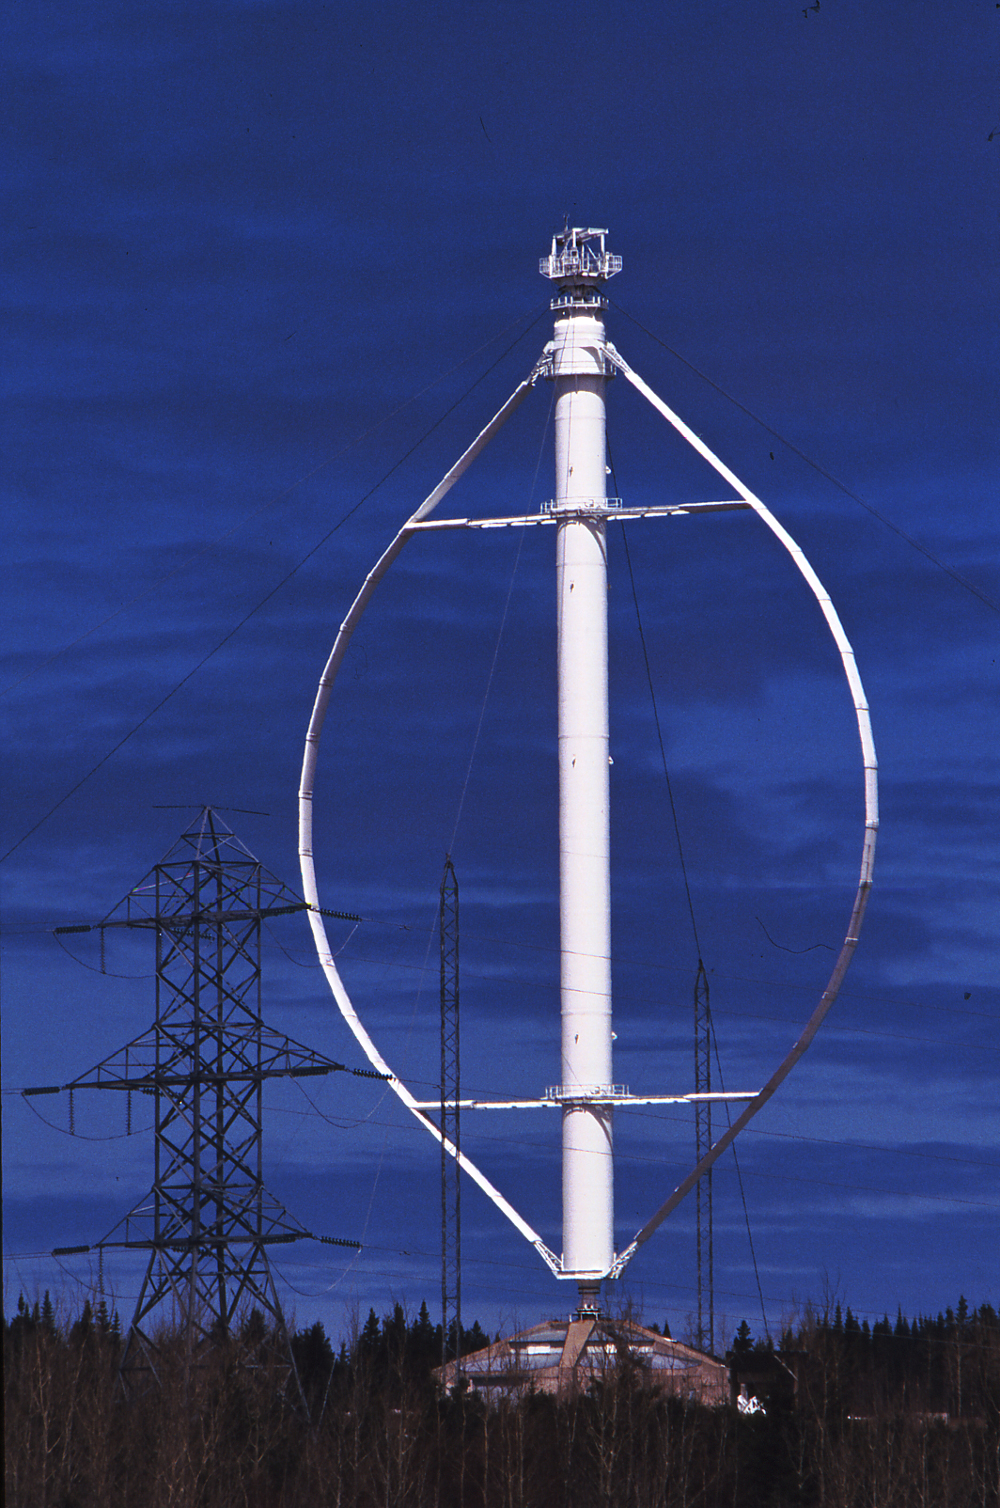
\includegraphics[clip, trim=0 0 0 0.2in, width=\textwidth]{Eole}
        
        \caption{Lavalin Eole 64 m VAWT.}
        
        \label{fig:Eole}
    \end{subfigure}
    
    \begin{subfigure}[b]{0.8\textwidth}
        \centering
        
        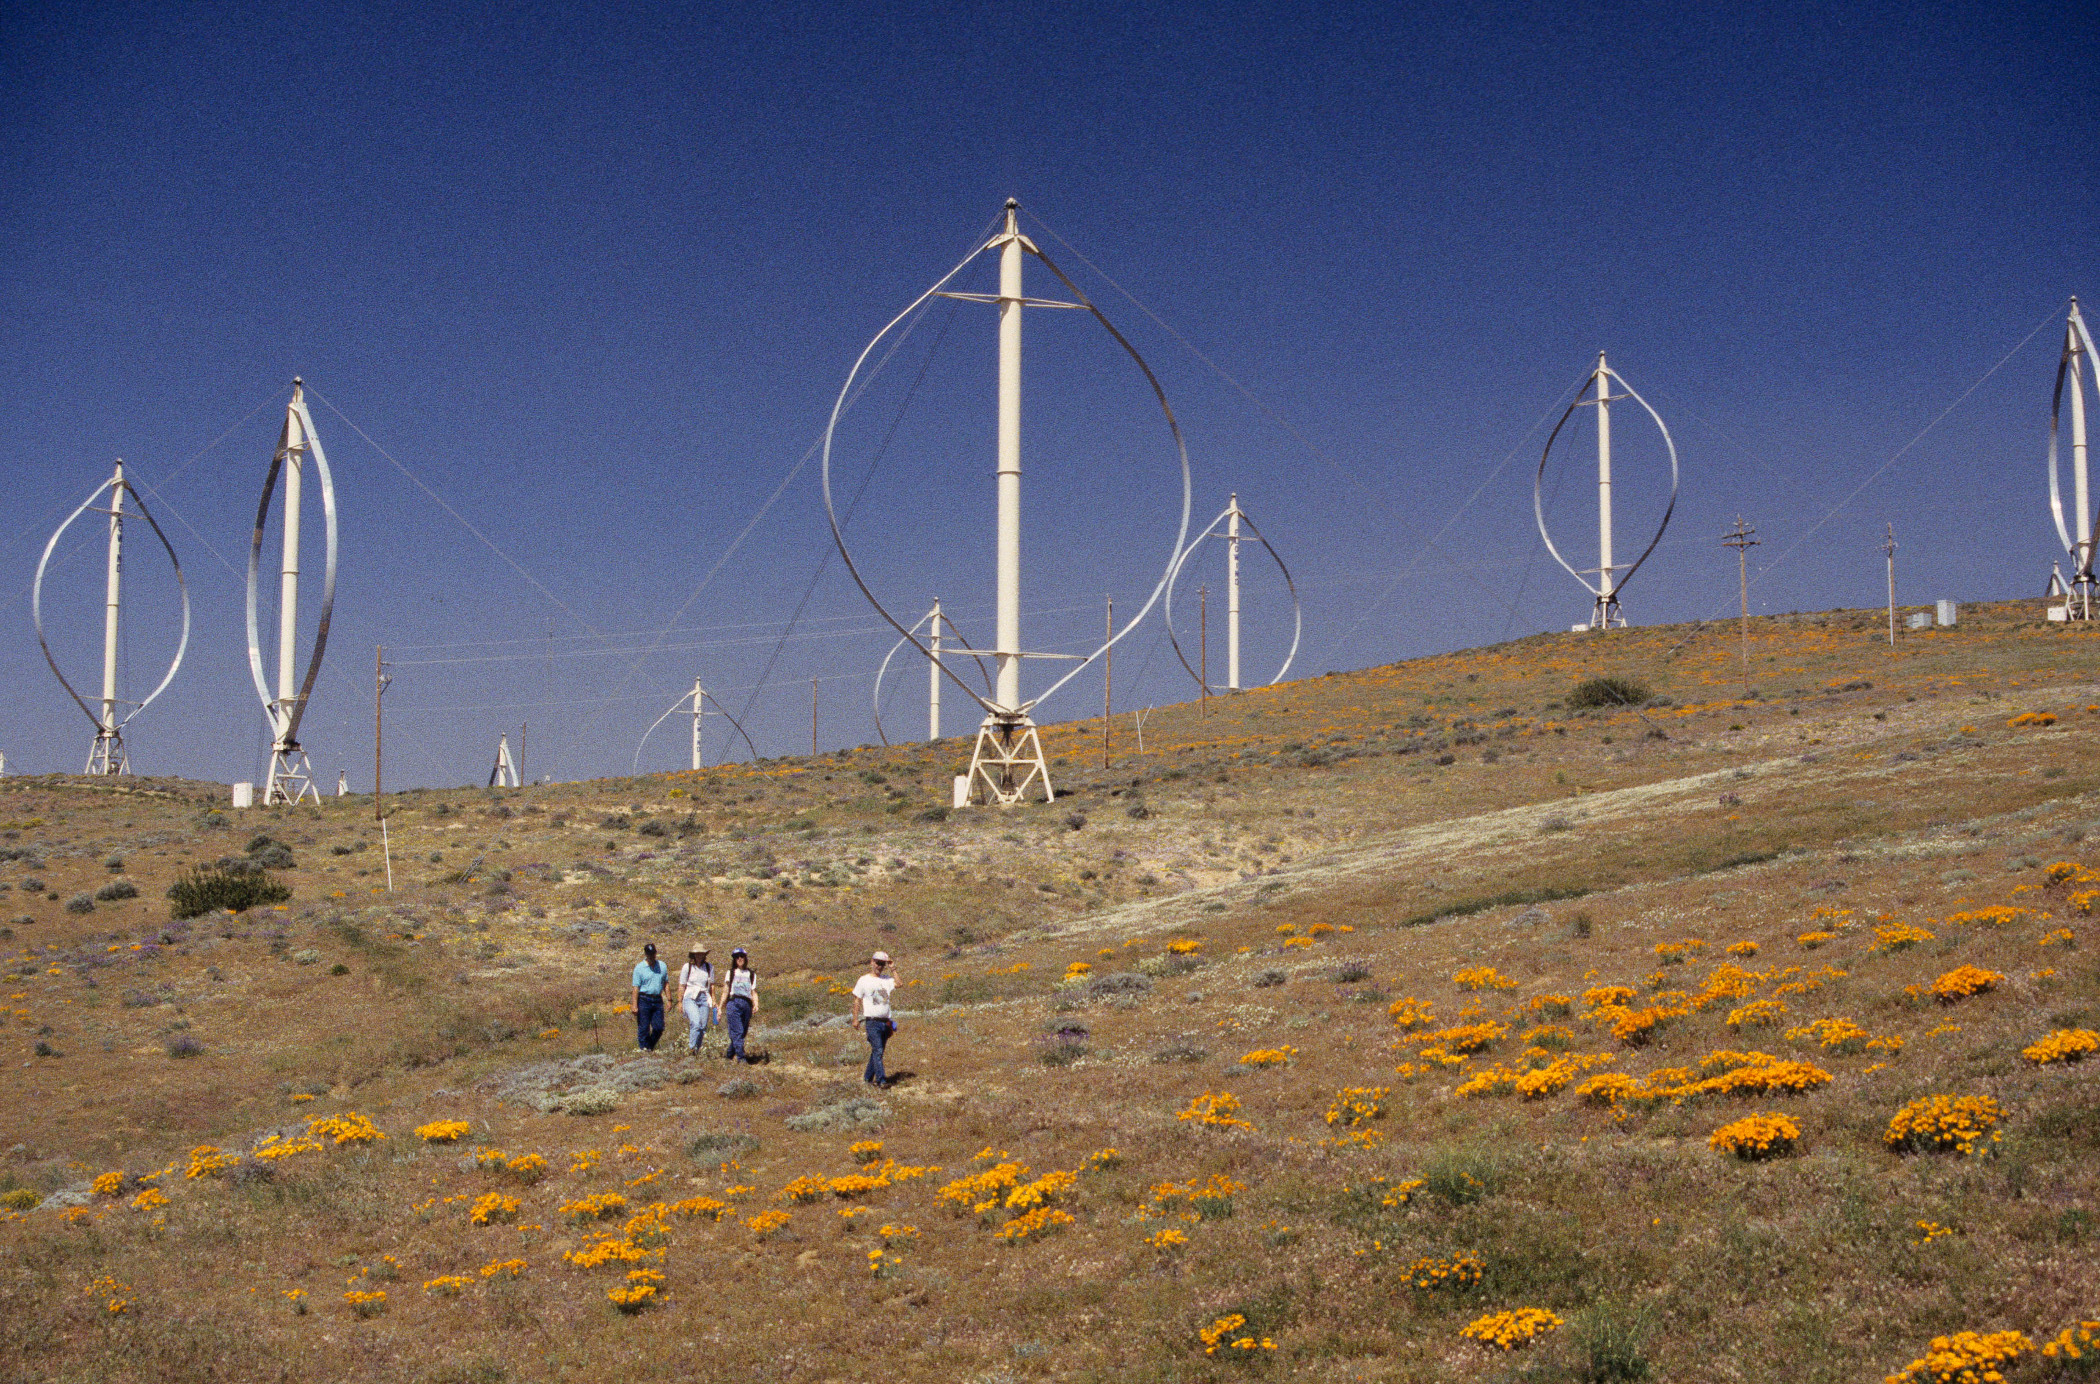
\includegraphics[width=\textwidth]{flowind}
        
        \caption{FloWind VAWT array.}
        
        \label{fig:FloWind}
    \end{subfigure}
    
    \caption{Large scale Darrieus wind turbines: Sandia 34 m Test Bed (a),
        Lavalin Eole 64 m (b), and FloWind VAWT array (c).}
    
    \label{fig:Darrieus}
\end{figure}


Ultimately the three-bladed, horizontal-axis propeller-type axial-flow turbine
(AFT) concept---shown in Figure~\ref{fig:AFT} has became the design of choice
for large scale onshore wind---and for good reasons. Axial-flow turbines are
easier to analyze since their operating principles can be though of as an
essentially steady flow over a foil before stall. AFTs also have the benefit of
research ``inertia''---a lot has been invested and a lot of knowledge has
accumulated already. As a result, the designs are quite mature, for wind energy
at least. In contrast, the CFT has been studied and applied significantly less,
though there have been cases where CFTs have performed nearly equivalently well
as AFTs. However, CFTs are harder to design, since their blades are constantly
changing their angles of attack throughout the turbine's rotation, often
undergoing dynamic stall as part of normal operation \cite{Para2002}. Beside
their unpredictability, the highly oscillatory blade loading presents
significant design challenges for avoiding fatigue---a main cause for failure or
premature retirement of the large Darrieus wind turbines.

\begin{figure}[ht]
    \centering
    
    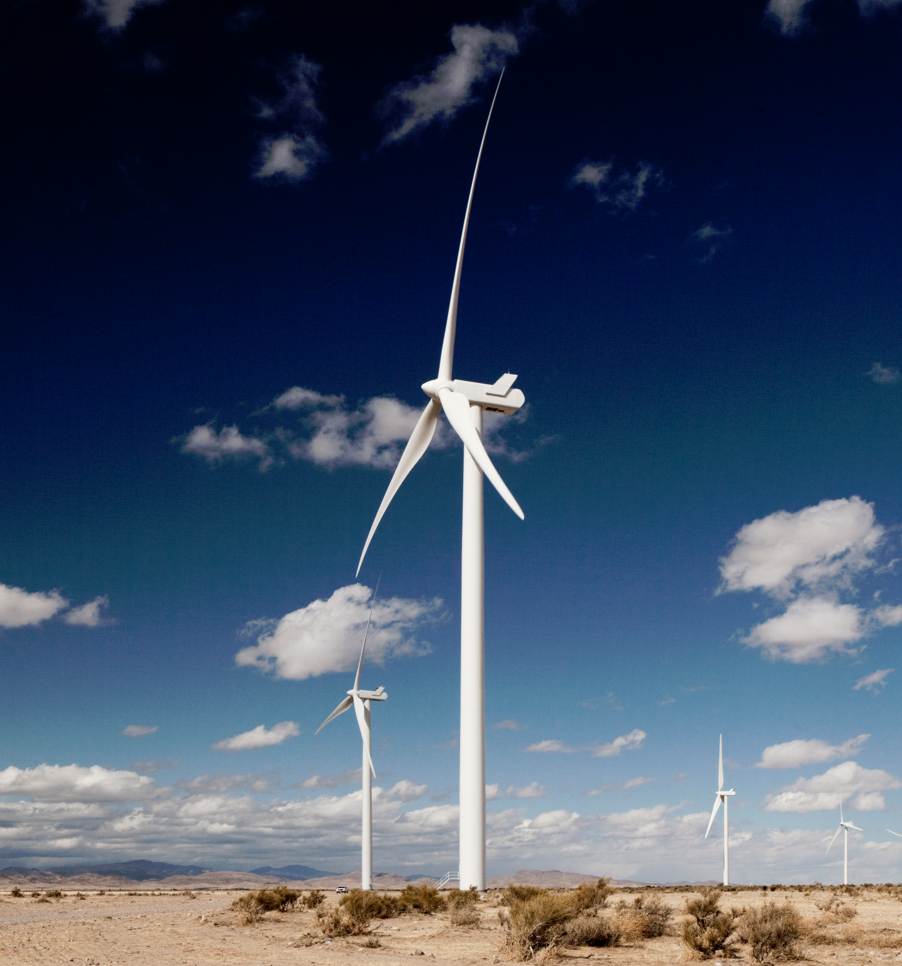
\includegraphics[width=0.7\textwidth]{Vestas-V100}
    
    \caption{Vestas V100 1.8 MW three-bladed axial-flow, a.k.a horizontal-axis
        wind turbine. Courtesy of Vestas Wind Systems A/S.}
    
    \label{fig:AFT}
\end{figure}

Despite their shortcomings, CFTs still may be valuable in some cases. They are
simpler, omni-directional machines, which negates the need for yawing and
pitching mechanisms. There were considerations in the 2010s by DEEPWIND in
Europe \cite{Paulsen2011} and SNL \cite{Sandia2012} in the US for using large
scale floating VAWTs for offshore wind, since along with the
omni-directionality, a vertical shaft allows placement of the generator and
gearbox lower in the machine, which lowers center of gravity. In the onshore
wind arena, CFTs show promise for projects where space is limited, e.g., urban
environments, as adjacent turbines sometimes interact ``constructively'' to
increase each other's power outputs \cite{Li2010}---a trait not possessed by
AFTs. A group from the California Institute of Technology has shown that arrays
of VAWTs can potentially provide an order-of-magnitude increase in the power
output per land area of a wind turbine array, since the devices can be spaced
more closely than HAWTs \cite{Dabiri2011}. Field measurements have shown that
their wakes recover more quickly than those of AFTs, and this cannot be entirely
attributed to higher turbulence generation \cite{Kinzel2012}. This phenomenon is
investigated in later chapters.

In the built, i.e., suburban and urban environments, wind resources are less
understood, more variable in terms of direction, speed, and turbulence levels
\cite{Smith2012}. Kooiman and Tullis \cite{Kooiman2010} observed that a
cross-flow turbine in an urban environment was indeed insensitive to changes in
wind direction, and was only adversely affected by temporal variations in wind
speed when turbulence intensity was above 15\%. The lack of need for yawing can
help lower cost of energy from CFTs versus AFTs by reducing complexity, e.g., by
eliminating slip rings. Cross-flow turbines may also have an advantage in the
urban environment since they must be designed for high fatigue loads anyway.
Recently, the Eiffel tower in Paris, France has been outfitted with two 5.3 m
tall, 3.2 m diameter helical vertical-axis cross-flow turbines, which will
produce at least 10 kWh/yr, or approximately 1 kW on average, which is expected
to power the entire first floor of the facility \cite{Lott2015}.

For MHK development, a field much less mature than wind power, the cross-flow
turbine concept is playing a major role thanks to its omni-directionality and
flexibility with respect to frontal area shape, allowing for more precisely
tuned fitment in channels with complex bathymetry or installed structures.
Chosen by the Ocean Renewable Power Company (ORPC) for their TidGen design, a
cross-flow turbine was the first grid-connected tidal energy device in the US,
which was installed in Cobscook Bay, ME \cite{ORPC2012}. Today, ORPC is working
on improving their turbine's performance, and planning for the installation of 4
more turbines \cite{Nelson2013}. CFTs are also being considered for micropower
applications, such as powering remote underwater instrumentation packages that
currently rely on batteries \cite{Polagye2013b}. As will be discussed in the
following section, present predictive capability is significantly less than
adequate, for both individual devices and arrays, which is a primary motivation
for this research.


\todo[inline]{Add more recent MHK stuff, e.g. Instream, Yakima, Gorlov, Lucid,
    RivGen}


\section{Principles of cross-flow turbine operation}

Blade element theory can be employed to obtain a simplified view of the
kinematics and dynamics of a CFT. Figure~\ref{fig:vectors} shows the relevant
velocity and and force vectors on a CFT blade element. The relative velocity and
angle of attack $\alpha$ are calculated by adding the inflow velocity vector to
the opposite of the blade element velocity $\omega R$, where $\omega$ is the
shaft angular velocity and $R$ is the element radius. In the relative velocity
coordinate system, the lift and drag are then oriented normal and tangential to
the relative velocity, respectively. These forces ultimately produce the shaft
torque, and in turn the shaft power. 

\begin{figure}[ht]
    \centering
    
    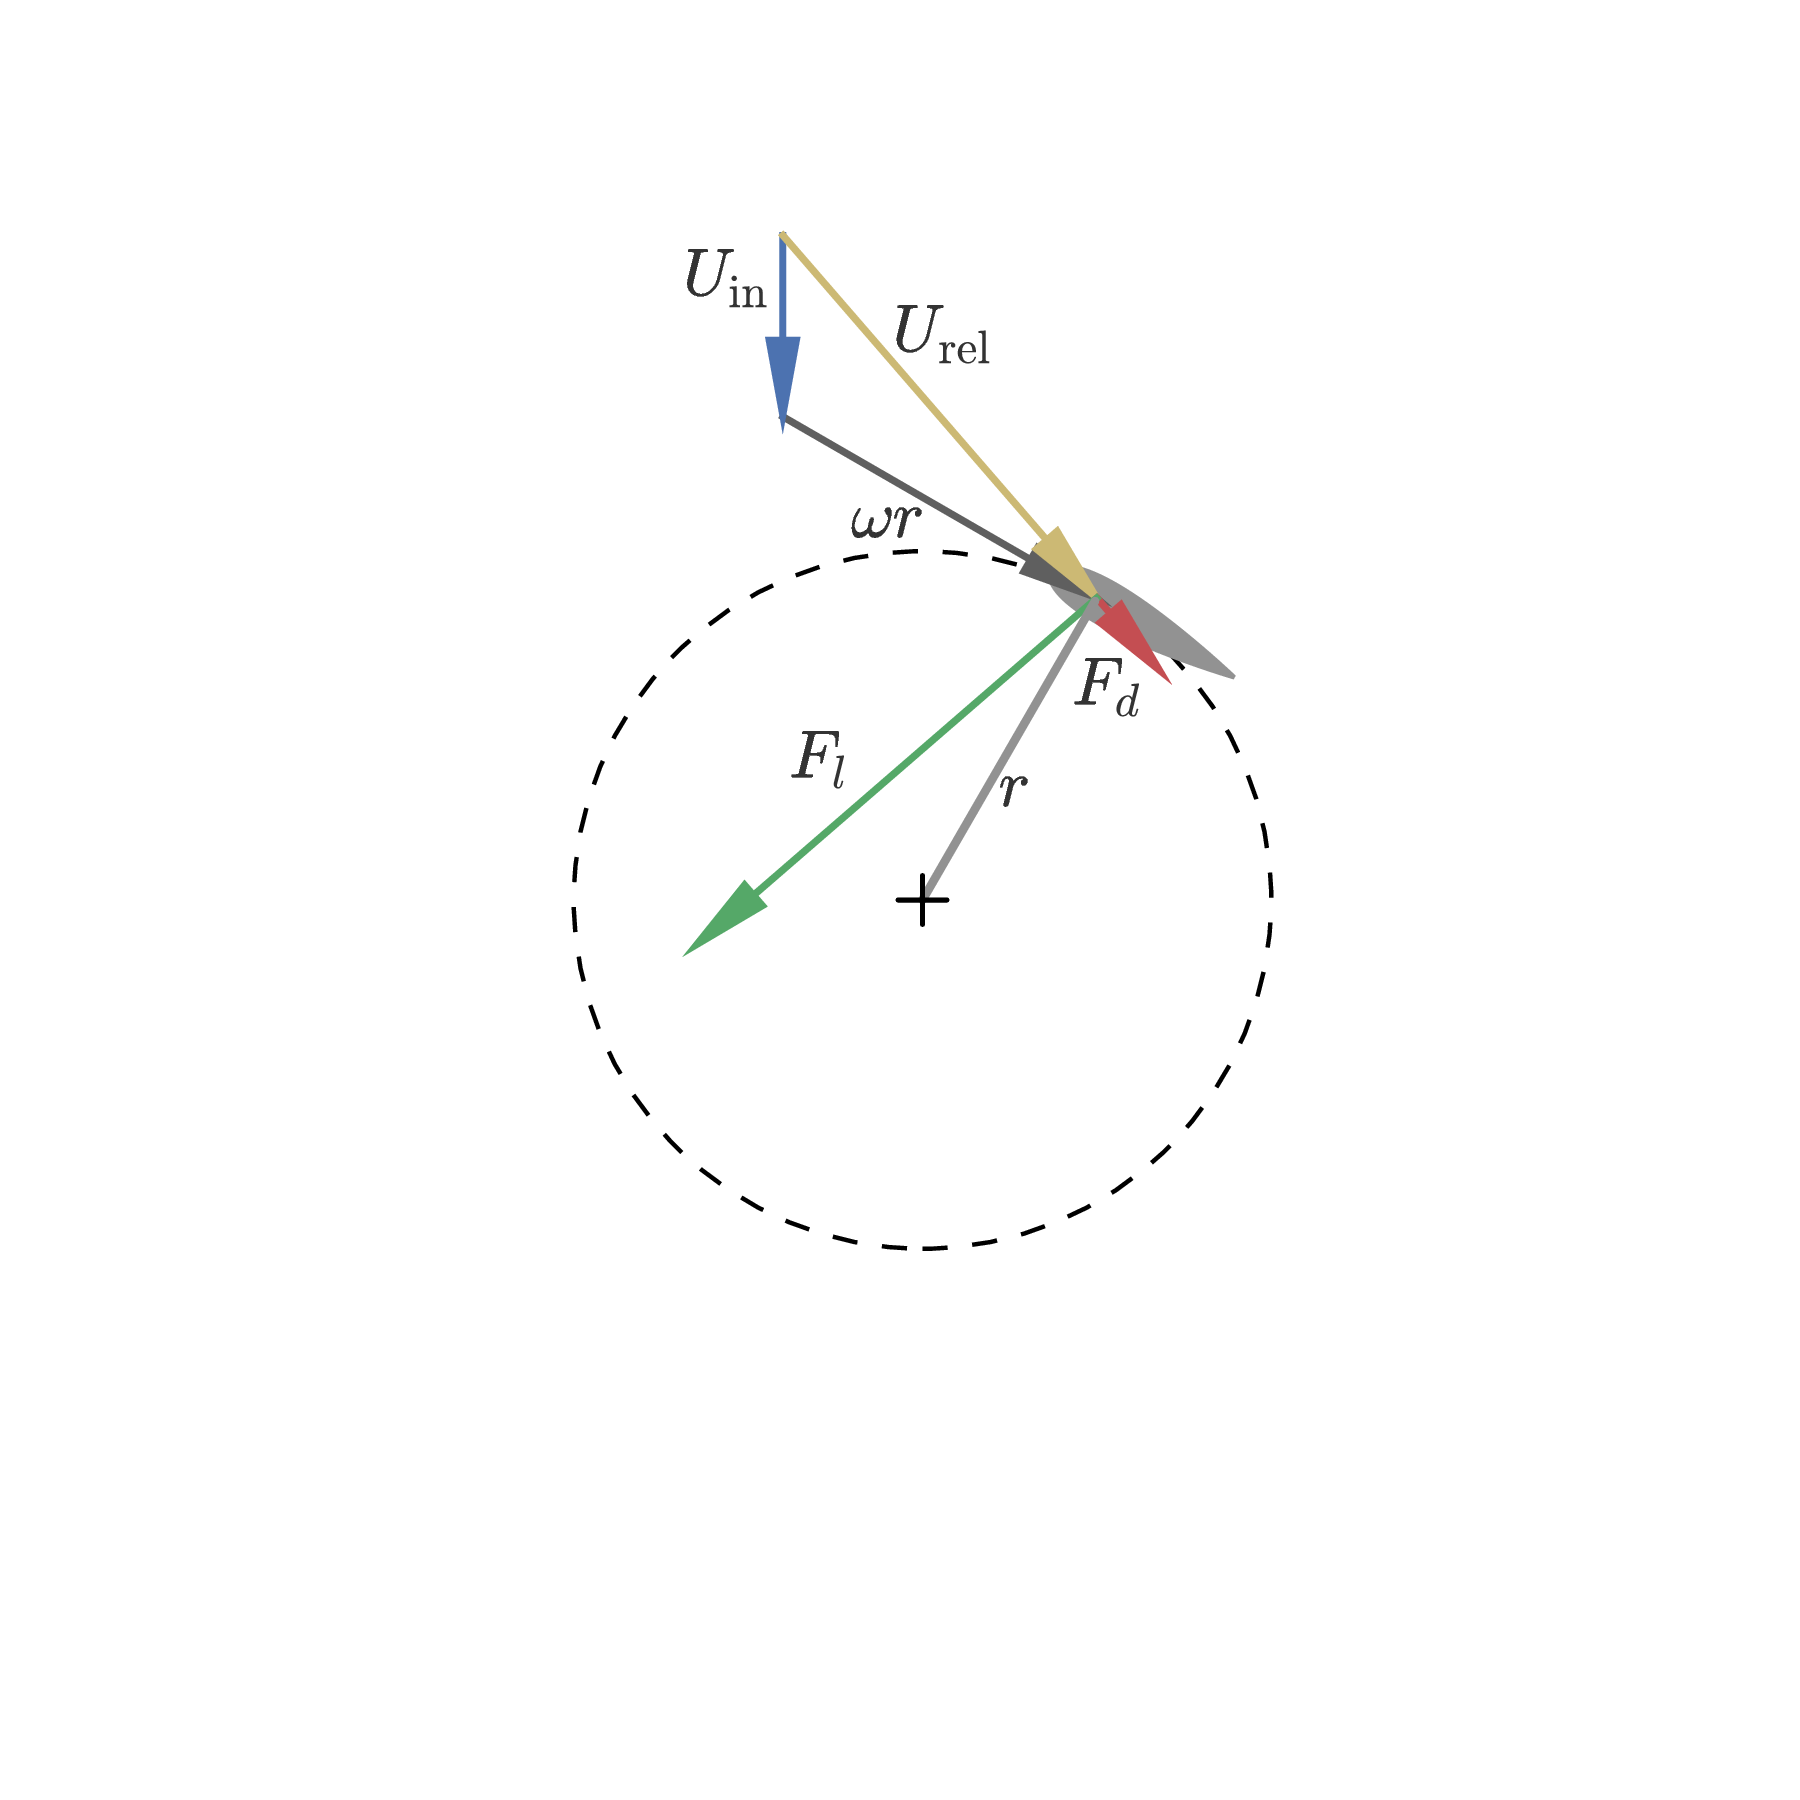
\includegraphics[clip, trim=1in 1.5in 1in 0.5in,
    width=0.6\textwidth]{figures/CFT-vectors_cft-vectors}
    
    \caption{Vector diagram of velocity and forcing on a cross-flow turbine
        blade element.}
    
    \label{fig:vectors}
\end{figure}

The shaft's angular velocity is nondimensionalized as the tip speed ratio
\begin{equation}
    \lambda = \frac{\omega R}{U_\infty},
    \label{eq:lambda}
\end{equation}
where $U_\infty$ is the free stream velocity.
Torque $T$ is characterized by the nondimensional torque coefficient 
\begin{equation}
    C_T = \frac{T}{\frac{1}{2} \rho A R U_\infty^2},
    \label{eq:ct}
\end{equation}
where $\rho$ is the fluid density and $A$ is the turbine's frontal area.
Similarly, the turbine power $P = T\omega$ and overall rotor drag $F_D$ are
normalized as the power coefficient
\begin{equation}
    C_P = \frac{T \omega}{\frac{1}{2} \rho A U_\infty^3},
    \label{eq:cp}
\end{equation}
and the rotor drag coefficient
\begin{equation}
    C_D = \frac{F_D}{\frac{1}{2} \rho A U_\infty^2}.
    \label{eq:cd}
\end{equation}
It is also worth noting that $C_P = \lambda C_T$.

So why then, is it difficult to analyze these machines? A first glimpse can be
seen in Figure~\ref{fig:geom-alpha-urel}, where the geometric angle of attack
and relative velocity are plotted over one turbine revolution for various tip
speed ratios. If we imagine a typical high solidity $\sigma = Nc/R$ turbine
operating at an optimal tip speed ratio $\lambda_0 = 2$, for example
\cite{Howell2010} (note that solidity and $\lambda_0$ are inversely correlated
\cite{Templin1974}), we see that angles of attack can be very high even in
optimal conditions. Keep in mind that we are calculating geometric angle of
attack---the ``true'' angle of attack will be reduced by a slowing of the inflow
velocity, also known as induction. 

\begin{figure}[ht]
    \caption{Geometric angle of attack and relative velocity versus azimuthal
        angle at various tip speed ratios.}
    
    \label{fig:geom-alpha-urel}
\end{figure}

As shown in Figure~\ref{fig:vectors}, the blade's lift to drag ratio and angle
of attack can be thought of as the quantities to maximize in order to develop
shaft torque. However, beyond a threshold angle of attack, i.e., the static
stall angle, $C_l/C_d$ drops. Predicting foil characteristics (lift, drag,
pitching moment) is difficult beyond the static stall angle, where boundary
layer separation becomes dominant over most of the foil suction surface, which
reduces lift and increases drag dramatically. For example,
Figure~\ref{fig:S826-perf} shows measured lift and drag coefficients compared
with 2-D and 3-D Navier--Stokes CFD simulations from Cakmakcioglu \etal
\cite{Cakmakcioglu2014}. The linear lift slope region and static stall angle are
predicted well enough, but the peak $C_l/C_d$ is massively overestimated. This
may not be an issue for a machine designed to operate at relatively fixed and/or
pre-stall $\alpha$, e.g., airplane wings, propellers, or axial-flow wind
turbines, but a cross-flow turbine will most likely encounter post-stall
regimes, making even high-fidelity CFD analysis an uncertain prospect for
accurate blade load prediction.


\begin{figure}[ht]
    \centering
    
    \includegraphics[width=\textwidth]{figures/cakmak-et-al-2014-fig8}
    
    \caption{Characteristics of an S826 airfoil at $Re=145,000$, from
        \cite{Cakmakcioglu2014}.}
    
    \label{fig:S826-perf}
\end{figure}


\todo[inline]{Show examples of XFOIL.} As we see, even simple tools based on
potential flow can do a good job predicting foil characteristics in the linear
regime, but as stall is encountered, numerical prediction becomes very difficult
due to the complex flow physics.


\subsection{Unsteady aerodynamics and dynamic stall}

Up until now we have only considered the static behavior of foils, which may be
sufficient to model the steady performance of an axial-flow turbine, since rotor
blade element angles of attack are meant to remain constant in ideal conditions.
The rotation of a cross-flow turbine, however---with its constantly changing
angle of attack (also the change in sign) and relative velocity---produces an
unsteady environment for the blade elements, even in an idealized case.

Unsteady foil behavior and dynamic stall have been studied extensively in
rotorcraft research. In the absence of stall, even a helicopter rotor airfoil
will deviate from static behavior due to cyclic pitching, along with changes in
relative velocity as the blade advances and retreats. Thus, the wealth of
knowledge available from the helicopter literature provides insight into the
cross-flow turbine case.

The first consideration is the attached behavior of unsteady airfoils. As one
might expect, in these cases either the angle of attack or relative velocity is
varying, but flow separation, i.e. stall, is never encountered.


\section{The state of engineering tools for CFTs}

\subsection{For individual devices}

Presently, the most reliable predictor of turbine performance is physical
modeling (building prototypes or copying existing designs that have been
field-tested), so long as important dynamical scales (Reynolds number, mainly)
are sufficiently matched. It has been shown that performance becomes essentially
Reynolds number independent at an approximate blade chord Reynolds number $Re_c
\approx \lambda U_\infty c / \nu = O(10^5)$ \cite{Bravo2007}, which was
confirmed by experiments with a reference turbine in the UNH tow tank
\cite{Bachant2014}. However, experiments at this scale can be quite expensive.
For example, a turbine with a 1 m diameter and 10 cm chord would need to be
tested in a flow on the order of 1 m/s in water and 10 m/s in air. For a turbine
this large it is typically impractical to manufacture many prototypes to find
the optimal design, so numerical modeling is preferred. There exists a large
spectrum of numerical modeling techniques with widely varying computational cost
and fidelity, and sometimes only the most complex and computationally expensive
are trustworthy.

Momentum models are the simplest and cheapest, where the turbine blades are
discretized into blade elements, for which 2-D static lift and drag data are
tabulated. The relative velocity and angle of attack for a blade element are
calculated by seeking a balance between forces computed from the static foil
data and the rate of change of momentum of the fluid passing by the blade
element. Momentum methods break down for large streamwise forces, i.e.,
``induction factors''---common in water and high solidity turbines---and must be
corrected empirically. Despite their deficiencies, these models can do a
reasonable job for low solidity (ratio of blade planform area to swept area)
turbines when combined with corrections for dynamic loading, the most prominent
cause of which is dynamic stall \cite{Para2002}. A double multiple streamtube
(DMS) momentum model can compute a full turbine performance curve in seconds on
a modern desktop computer.

Vortex line methods are similar to momentum models, except blade element local
velocity is computed using potential flow theory, where lifting bodies are bound
vortex lines that shed vortex wake elements whose influences are combined via
the Biot--Savart law \cite{Strickland1979}. Sandia National Labs' CACTUS is an
example of a vortex method \cite{Murray2011}. CACTUS has been tested against
experimental data from large, low-solidity wind turbines (those for which
momentum models do well), but has been shown to fail for smaller turbines in
water, which are typically higher solidity \cite{Michelen2014}. Regarding
computing effort, vortex line methods can compute a full turbine performance
curve in minutes---slightly longer than the DMS method, but still quite fast.
The increase in accuracy of the flow field prediction and the robustness with
respect to high turbine loading justify the slightly higher expense of the
vortex line method.

A more sophisticated vortex model is the so-called panel method, where turbine
geometry can be specified arbitrarily as potential flow boundary elements,
negating the need for sectional foil coefficient tables. This is a significantly
more computationally expensive model. A single turbine operating point (not a
curve) may take hours on a conventional desktop PC. Furthermore, boundary layer
models are necessary to predict the occurrence and consequences of dynamic
stall \cite{Zanon2012}.

The most computationally expensive models solve the Navier--Stokes equations,
with turbulence modeled with Reynolds-averaging (RANS) or large eddy simulation
(LES)---the former being relatively less expensive, since LES directly solves a
larger portion of the energy spectrum of turbulence. If a body-fitted grid is
used, the actual turbine geometry is included as part of the computational
domain, and the mesh is generally refined next to the solid surfaces to resolve
the boundary layer, i.e., with cells adjacent to walls having a nondimensional
wall distance $y^+ \sim 1$. When only run in two dimensions, RANS methods are
affordable enough to be run on a single CPU, computing a single turbine
operating point in hours. However, 3-D effects are important enough that 2-D
simulations are not reliable, at least as predictors of absolute performance
\cite{Li2013}. 3-D simulations with a body-fitted grid are very expensive
(especially for LES), therefore are practically limited to high performance
computing (HPC) clusters. Even with the high computational expense, these models
are not perfect and results can deviate significantly from experimental
measurements, especially when using RANS models \cite{Li2013}.

Actuator line models (ALMs) are a mixture of the blade element and
Navier--Stokes methods. The turbine is not part of the mesh, but is represented
by lines that move through the flow, acting as momentum sinks, where the
resultant force is computed using 2-D foil data. Negating the need for a
body-fitted grid and resolving the boundary layer removes a significant amount
of computational effort, but the flow field is still computed more accurately
than with momentum or vortex methods, since nonlinear effects and turbulence are
included in the RANS or LES equations.


\subsection{For arrays}

Effective turbine array engineering directly depends on accurate prediction of
turbine wake generation, evolution and interaction, along with the impact of
various types of turbulent inflow on power production of each device. Like for
individual turbines, physical modeling is an option for predicting array
performance, though it becomes even more expensive to match relevant dynamical
scales. For this reason, turbine arrays are mainly designed using numerical
methods.

The contemporary industry standard method for predicting array performance
involves the superposition of prescribed wakes \cite{Stevens2014b}. Evolution
can be dependent on a single expansion coefficient chosen by the free stream
turbulence intensity \cite{Jensen1983, Choi2013} or computed by a solution of
the linearized RANS equations with an empirically derived constant eddy
viscosity closure \cite{Ainslie1988}. In light of the CFT's unique near-wake
dynamics, the valitidy of these models is questionable. At the very least they
would need to be recalibrated for CFTs, though their applicability is limited in
the near-wake of any turbine, meaning they are generally inappropriate for
closely-spaced arrays.
	
The next step up in complexity is the actuator disk method, where a constant
body force is added to the Navier--Stokes equations. This method can be
computationally cheap with RANS, or quite expensive and thorough with LES. The
ORPC turbine array is being laid out using the SNL-EFDC code, which uses a
constant uniform force applied to the RANS equations, where the turbine injects
turbulence kinetic energy and dissipation for the model's $k$--$\epsilon$
closure \cite{Nelson2013}. These models will most likely fail to predict the
fast wake recovery of CFTs, as they do not resolve the blade forces that create
the unique mean flow field in the near-wake \cite{Bachant2015-JoT}.
	
At present simulations with body-fitted grids are limited to one or two turbines
due to computational cost, which means they are impractical for full array
simulations. Thus the actuator line method, when combined with LES, is the most
complex model being used today. The ALM has the benefit of resolving unsteady
flow features created by periodic blade forcing and end effects, ultimately
producing the most accurate parameterization for turbine induced forces in
Navier--Stokes simulations. It has been shown in blind axial-flow turbine
modeling tests that ALM/LES methods fair better when predicting turbine induced
turbulence, and therefore will be more accurate at predicting flow within a
turbine array \cite{Krogstad2013}.


\section{Goals and objectives}

At the most basic level, the goal this research is working towards is the
ability to predict the performance of and flow though an array of cross-flow
turbines, to allow for the evaluation of array layouts, and the prediction of
overall power output and potential environmental effects. The strategy for
meeting this goal includes the following objectives:

\begin{enumerate}

	\item To improve the understanding of both high and low solidity cross-flow
    turbine wakes, most importantly the apparent increased rate of recovery
    compared with axial-flow turbines. This will establish our flow modeling
    targets.
	
	\item To assess the allowable scale mismatch at which physical models can
	provide results relevant to full-scale devices and arrays.
	
	\item To evaluate the ability of high-fidelity computational fluid dynamics and
	high performance computing to supplement or even replace experimental work.
    
    \item To investigate the actuator line force parameterization to potentially
    reduce the required computing power necessary for engineering work with
    CFTs.
\end{enumerate}

To obtain a closer look at what is happening in the flow field around the RVAT,
3-D RANS simulations of the actual turbine geometry are being performed using
SNL's Red Mesa HPC cluster. If these simulations can correctly postdict the
blade loading and near-wake measurements, they can be used to ``interpolate''
the experimental results and provide more insight for validation of the ALM, or
to possibly diagnose and remedy some of the flaws within the CACTUS code.
Currently some test simulations have been run, showing promising results, and a
2-D slice of the model is being used to check for grid convergence.

As described in the previous section, the actuator line model is valuable in
that it can be used to predict both the performance and wake of a turbine. It
can also be applied to high fidelity modeling of turbine arrays thanks to its
time-resolved nature. The ALM also eliminates the need for complex grids, which
is a significant simplification since mesh generation is arguably the largest
impediment to automation in CFD \cite{Slotnick2014}. Computational effort will
also be significantly reduced since the ALM does not need a rotating mesh, and
small cells near the turbine blade surface can be eliminated.

The proposed model will have some of the drawbacks of momentum and vortex
methods for predicting performance, namely the reliance on static foil data.
However, the flow field, and therefore relative velocity and blade angle of
attack will be predicted more accurately, and should therefore produce more
accurate predictions of turbine performance and wake characteristics.

In a way, this research plan is ``backwards,'' i.e., the results are acquired
before the predictive models are implemented, which may produce a model with
limited applicability. However, an attempt is made to test the robustness of the
model by applying to two cases with disparate parameters.

Despite CFTs being somewhat rare in industry, the flow problem is complex yet
general enough to applicable to other unsteady turbomachinery and/or foil flows,
e.g., Voith Schneider propellers, Cyclogyros, or even conventional helicopter
rotors.


